\subsubsection{Scopo}
Lo scopo di questo processo consiste nell'illustrazione di come deve essere redatta e mantenuta
la documentazione, durante il \gl{ciclo di vita} del \gl{software}.
\subsubsection{Aspettative}
Le aspettative della corretta implementazione di tale processo sono:
\begin{itemize}
	\item una chiara visione della documentazione prodotta durante il ciclo di vita
del software;
	\item una serie di norme per la stesura di documenti coerenti e validi;
	\item una documentazione formale e coerente.
\end{itemize}
\subsubsection{Descrizione}
In questo documento devono essere redatte tutte le norme e le convenzioni adottate dal gruppo,
in modo da produrre una documentazione valida e coerente.
\subsubsection{Struttura dei documenti}
 \paragraph{Frontespizio}
La prima pagina di ogni documento dovrà contenere:
\begin{itemize}
	\item logo del gruppo;
	\item nome del \gl{progetto};
	\item nome del documento e la relativa versione;
	\item sommario;
	\item data di redazione;
	\item nome e cognome dei redattori del documento;
	\item nome e cognome dei \gl{verifica}tori del documento;
	\item nome e cognome del responsabile per l'approvazione del documento;
	\item uso del documento (interno o esterno);
	\item lista di distribuzione del documento.
\end{itemize}
 \paragraph{Diario delle modifiche}
 La seconda pagina dovrà contenere il diario delle modifiche di quel determinato documento.\\
 Il diario è costituito di una tabella ordinata in modo decrescente seconda la data di modifica e il numero di versione.\\
 Gli attributi della tabella rappresentano:
 \begin{itemize}
 	\item numero di versione;
 	\item breve riepilogo delle modifiche apportate;
 	\item autore delle modifiche;
 	\item ruolo ricoperto dall'autore all'interno del progetto;
 	\item data di modifica.
 \end{itemize}
 \paragraph{Indici}
 In ogni documento è presente un indice delle sezioni, utile a fornire una visione macroscopica della struttura del documento. Sono previsti, se necessari, gli indici relativi alle tabelle e alle figure presenti nel documento in questo ordine.
 
 \paragraph{Intestazione e piè di pagina}
L'intestazione delle pagine di ogni documento deve contenere:
\begin{itemize}
	\item numero e titolo della sezione;
	\item nome del progetto.
\end{itemize}
Il piè di pagina contiene invece:
\begin{itemize}
	\item nome del documento con la relativa versione;
	\item nome del gruppo;
	\item pagina X di Y, dove X è la pagina corrente e Y è il numero di pagine totali del documento.
\end{itemize}
\paragraph{Introduzione}
In questa sezione vengono fornite le seguenti informazioni: 
\begin{itemize}
	\item scopo del documento;
	\item glossario;
	\item riferimenti utili;
	\begin{itemize}
		\item riferimenti normativi;
		\item riferimenti informativi.
	\end{itemize}
\end{itemize}
\subsubsection{Norme tipografiche}
In questa sezione vengono definite le norme ortografiche e tipografiche da rispettare nella stesura di ogni documento.
 \paragraph{Stile del testo}
 Al fine di migliorare la leggibilità e comprensione di un documento, è d'obbligo preferire uno stile d'esposizione sfruttando elenchi piuttosto che uno stile narrativo, in maniera tale da esporre i contenuti più esplicitamente.	
\begin{itemize}
	\item \textbf{Grassetto}: viene utilizzato per:
	\begin{itemize}
		\item titoli;
		\item elementi di un elenco puntato che riassumono il contenuto del relativo paragrafo.
	\end{itemize}
	\item \textbf{Corsivo}: viene utilizzato per:
	\begin{itemize}
		\item citazioni;
		\item abbreviazioni;
		\item parole inserite nel glossario;
		\item riferimenti ad altri documenti;
		\item nomi di società o aziende;
		\item ruoli dei membri del gruppo.
	\end{itemize}
	\item \textbf{Maiuscolo}: le parole scritte interamente in maiuscolo dovranno riferirsi soltanto ad acronimi.
	\item \textbf{Monospace}: le porzioni di testo scritte in monospace definiscono:
	\begin{itemize}
		\item frammenti di codice;
		\item comandi;
		\item \gl{URL}.
	\end{itemize}
	\item \textbf{Glossario}: le parole che hanno un riferimento nel glossario sono in corsivo e hanno una 'g' a pedice.
\end{itemize}
\subparagraph{Righe mal poste}
Le righe mal poste sono quelle righe che coincidono con una delle seguenti descrizione:
\begin{itemize}
	\item una riga di un paragrafo (o un titolo di livello superiore o inferiore) che inizia alla fine di una pagina;
	\item una riga di un paragrafo (o un titolo di livello superiore o inferiore) che finisce all'inizio di una pagina.
\end{itemize}
Per una questione di leggibilità, queste tipologie di righe devono essere evitate.\\
 L'utilizzo del comando \LaTeX{} \file{\textbackslash{newpage}} aiuta a risolvere questo problema.
 \subparagraph{Virgolette}
 I vari tipi di virgolette devono essere usati nei seguenti modi:
 \begin{itemize}
 	\item \textbf{Virgolette singole ' '}: devono essere utilizzate solo per racchiudere un singolo carattere;
 	\item \textbf{Virgolette doppie " "}: devono essere utilizzate solo per racchiudere:
 	\begin{itemize}
 		\item citazioni;
 		\item nomi di documenti;
 		\item voci di un menù;
 		\item voci di pulsanti da premere.
 	\end{itemize}
 \end{itemize}
 \paragraph{Elenchi puntati}
Tutti gli elenchi puntati sono caratterizzati graficamente da un pallino nel primo livello, da una trattino nel secondo e da un asterisco nel terzo (automatizzato grazie al \gl{template} \LaTeX{}{} creato). \\
Ogni elemento deve terminare con il punto e virgola, a meno che non sia l'ultimo dell'elenco, in questo caso la frase va terminata con il punto. Ogni punto inizia con la minuscola, tranne nel caso in cui necessiti di una spiegazione: allora
si utilizzerà la maiuscola.\\
Il seguente esempio vuole chiarire la differenziazione grafica tra i vari livelli di un elenco.
\begin{itemize}
	\item primo livello;
	\begin{itemize}
		\item secondo livello;
		\begin{itemize}
			\item terzo livello;
		\end{itemize}
		\item secondo livello;
	\end{itemize}
	\item primo livello.
\end{itemize}
 \paragraph{Formati comuni}
\begin{itemize}
	\item \textbf{Date}:\\ \\ \centerline{AAAA - MM - GG} \\ \\
	dove:
	\begin{itemize}
		\item AAAA: rappresenta l'anno utilizzando 4 cifre;
		\item MM: rappresenta il mese utilizzando 2 cifre;
		\item GG: rappresenta il giorno utilizzando 2 cifre.
	\end{itemize}
	Ad esempio, 2016-12-01 è una data scritta secondo le norme stabilite;
	\item \textbf{Orari}:\\ \\ \centerline{HH:MM} \\ \\dove:
	\begin{itemize}
		\item HH: rappresenta l'ora e può assumere valori da 0 a 23;
		\item MM: rappresenta i minuti e può assumere valori da 0 a 59.
	\end{itemize}
	Ad esempio, 15:05 è un orario scritto secondo le norme stabilite;
	\item \textbf{Nomi ricorrenti}:
	\begin{itemize}
		\item \textbf{Ruoli di progetto}: ogni nome di un ruolo di progetto deve essere scritto con la lettera iniziale maiuscola e con lo stile corsivo. Questo viene automatizzato utilizzando il comando \file{\textbackslash{CodiceRuolo}};
		\item \textbf{Nomi propri}: ogni nome deve essere espresso nella forma "Nome Cognome";
		\item \textbf{Nomi dei documenti}: ogni nome di documento viene scritto con lo stile corsivo, con l'iniziale di ogni parola maiuscola e con la versione corrente. Questo viene automatizzato richiamando il comando \file{\textbackslash{SiglaDocumentodoc}}.
	\end{itemize}
	\item \textbf{URL}: un URL dovrà essere scritto in azzurro ed essere un collegamento alla risorsa a cui punta e, per rendere automatizzato questo stile, si deve far utilizzo del comando \file{\textbackslash{url}}.\\
	Ad esempio, \url{https://www.google.it/} (visitato in data 2017-02-24) è scritto secondo le norme stabilite.
\end{itemize}
 \paragraph{Sigle}
E' previsto l'utilizzo di queste sigle:
\begin{itemize}
	\item \textbf{AdR}: per \ARdoc;
	\item \textbf{PdP}: per \PPdoc;
	\item \textbf{NdP}: per \NPdoc;
	\item \textbf{SdF}: per \SFdoc;
	\item \textbf{PdQ}: per \PQdoc;
	\item \textbf{ST}: per \STdoc;
	\item \textbf{Gl}: per \Gldoc;
	\item \textbf{DP}: per \DPdoc;
	\item \textbf{Rp}: per \RESP;
	\item \textbf{Am}: per \AMM;
	\item \textbf{Pt}: per \PJ;
	\item \textbf{An}: per \AN;
	\item \textbf{Pm}: per \PR;
	\item \textbf{Ve}: per \VER;
	\item \textbf{RR}: per \textbf{Revisione dei requisiti};
	\item \textbf{RP}: per \textbf{Revisione di progettazione};
	\item \textbf{RQ}: per \textbf{Revisione di qualifica};
	\item \textbf{RA}: per \textbf{Revisione di accettazione}.
\end{itemize}
L'utilizzo di queste sigle è permesso all'interno di:
\begin{itemize}
	\item tabelle;
	\item diagrammi;
	\item immagini;
	\item didascalie.
\end{itemize}
\paragraph{Nomi}
\subparagraph{Ruoli}
Quando si fa riferimento ad un ruolo di progetto bisogna adottare lo stile corsivo e la prima lettera deve essere maiuscola. \\
Per automatizzare ciò, si deve far utilizzo dei comandi \LaTeX{} definiti in \REF.
\subparagraph{Periodi}
Quando si fa riferimento ad un periodo del progetto bisogna utilizzare i comandi \LaTeX{} definiti in \REF.
\subsubsection{Elementi grafici}
 \paragraph{Tabelle}
 Al fine di facilitarne la tracciabilità, le tabelle devono essere:
 \begin{itemize}
 	\item in netto stacco rispetto i paragrafi che seguono e precedono;
 	\item accompagnate da una didascalia;
 	\item accompagnate da un numero incrementale;
 	\item centrate nella pagina.
 \end{itemize}
 \paragraph{Immagini}

Al fine di facilitarne la tracciabilità, le immagini devono essere:
\begin{itemize}
	\item in netto stacco rispetto i paragrafi che seguono e precedono;
	\item accompagnate da una didascalia;
	\item accompagnate da un numero incrementale;
	\item centrate nella pagina;
	\item essere di formato PNG.
\end{itemize}
\subsubsection{Classificazione dei documenti}
 \paragraph{Documenti informali}
 Tutti i documenti sono da ritenersi informali fino all'approvazione da parte del \RESP{} di progetto, ed in quanto tali sono da considerarsi esclusivamente ad uso interno.
 \paragraph{Documenti formali}
 Un documento viene definito formale quando viene validato dal \RESP{} di progetto. Solo i documenti formali possono essere distribuiti all'esterno del gruppo. Per arrivare a tale stato il
documento deve aver passato la verifica e la \gl{validazione}.
 \paragraph{Glossario}
Il glossario nasce dall'esigenza di chiarire il significato di parole che possono risultare ambigue all'interno di determinati contesti. Saranno quindi presenti parole che:
\begin{itemize}
	\item trattano argomenti tecnici;
	\item possono creare delle ambiguità sul significato;
	\item rappresentano delle sigle.
\end{itemize}
La struttura deve avere queste caratteristiche:
\begin{itemize}
	\item le parole devono essere in ordine alfabetico;
	\item ogni termine deve essere seguito da una spiegazione chiara e concisa, che non generi alcun tipo di ambiguità.
\end{itemize}
 \paragraph{Verbali}
Questo documento ha lo scopo di riassumere in modo formale le discussioni effettuate e le decisioni prese durante le riunioni. I verbali, come le riunioni, sono classificati in: interni ed esterni. In
particolare i verbali esterni, essendo documenti ufficiali, devono essere redatti dal \RESP{} di Progetto. I verbali interni, invece, dovranno essere redatti dagli \AMMP{}. \\
Ogni verbale dovrà essere denominato nel seguente modo:\\ \\
\centerline{\textit{Verbale\textunderscore{TipoVerbale}\textunderscore{DataVerbale}}}
\\ \\
dove:
\begin{itemize}
	\item \textbf{TipoVerbale}: identifica se il verbale è riferito ad una riunione interna (I) o esterna (E);
	\item \textbf{DataVerbale}: identifica la data nella quale si è svolta la riunione relativa al verbale.
\end{itemize}
Nella parte introduttiva vengono specificate le seguenti informazioni:
\begin{itemize}
	\item luogo di incontro;
	\item data di incontro;
	\item orario di inizio;
	\item orario di fine;
	\item durata dell'incontro;
	\item oggetto dell'incontro;
	\item partecipanti;
	\item segretario;
	\item segnalazioni varie.
\end{itemize}
Tutte le decisioni prese durante la riunione vengono identificate univocamente utilizzando questo formato: \\ \\
\centerline{\textbf{DIX.Y} per i verbali interni}  \\ \\
\centerline{\textbf{DEX.Y} per i verbali esterni}  \\ \\
dove:
\begin{itemize}
	\item \textbf{X}: rappresenta il numero di verbale redatto in ordine cronologico (inizia da 1);
	\item \textbf{Y}: rappresenta il numero della decisione all'interno di un singolo verbale (inizia da 1).
\end{itemize}
Inoltre vengono tracciate le decisioni in sospeso che verranno chiarite in verbali successivi. Il formato identificativo è lo stesso delle decisioni definitive, dove nel codice la D viene sostituita dalla S.
\subsubsection{Procedure}
Per la stesura della documentazione si è utilizzato il linguaggio \LaTeX{}, si veda la \hyperref[sec:Strumenti]{sezione strumenti \ref*{sec:Strumenti}}.
\paragraph{Approvazione dei documenti}
La formalizzazione di un documento segue la seguente procedura:
\begin{enumerate}
	\item il documento viene redatto da coloro che sono incaricati della sua stesura ed eventuale correzione di errori;
	\item per ogni significativa modifica del documento, i \VERP{} avranno il compito di controllare la presenza di errori o imprecisioni;
	\item se i \VERP{} riscontrano degli errori, dovranno notificarlo ai redattori del documento tramite una specifica \gl{issue}, tornando così al punto 1, altrimenti, se completo, il documento viene consegnato al \RESP{};
	\item il \RESP{} di progetto decide se approvare, e quindi formalizzare il documento, oppure se rifiutarlo comunicando la motivazione e le modifiche da apportare, tornando così al punto 1.
\end{enumerate}
\begin{figure}[h]
	\centering
	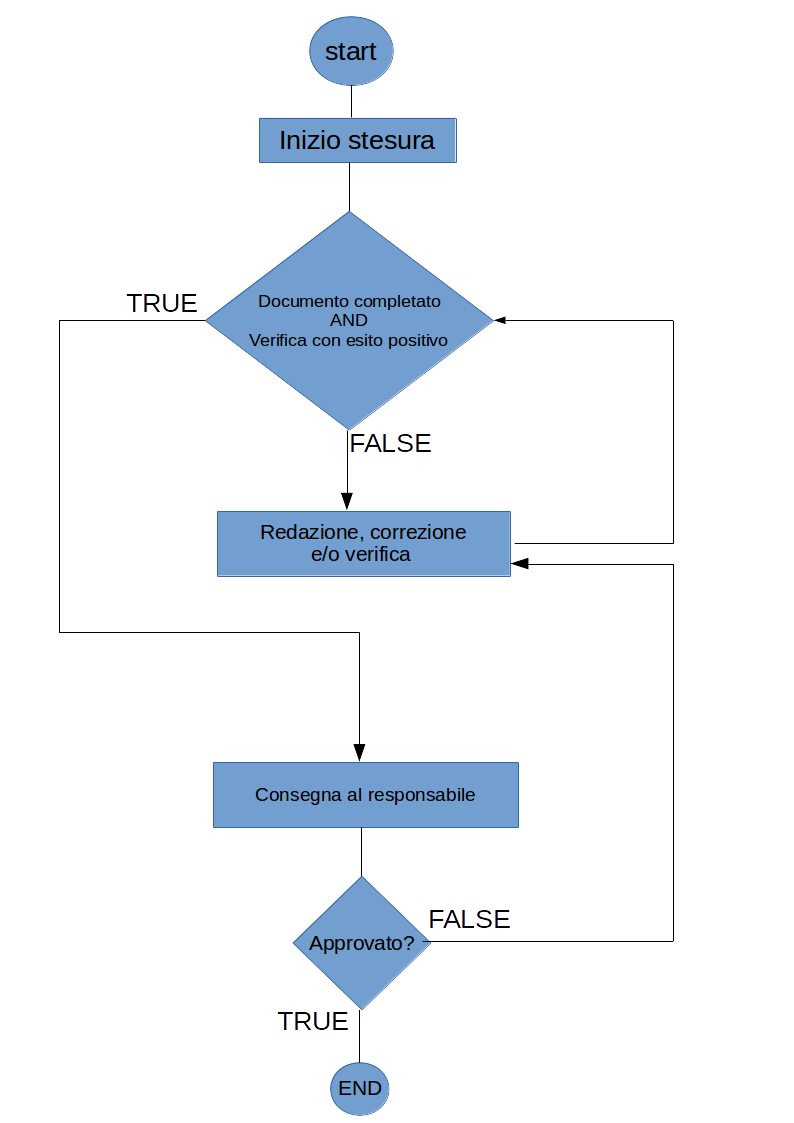
\includegraphics[scale=0.4]{img/flussoapprovazione.png}
	\caption{Flow chart dell'approvazione di un documento}\label{sec:Figura2}
\end{figure}

\newpage
\paragraph{Versionamento}
Ciascun documento che verrà redatto dovrà essere versionato, per consentire un tracciamento chiaro della sua storia e delle sue modifiche.\\Verrà applicato il seguente formalismo:\\ \\ \centerline{vX.Y.Z}\\ \\dove:
\begin{itemize}
	\item \textbf{X}:
	\begin{itemize}
		\item inizia da 0;
		\item viene incrementato quando il \RESP{} di progetto approva il documento. Per ogni periodo (vedi RIFERIMENTO PDP, capitolo 3), ci sarà una approvazione di ogni documento.
	\end{itemize}
	\item \textbf{Y}:
	\begin{itemize}
		\item inizia da 0;
		\item viene incrementato dal \VER{} ad ogni verifica;
		\item quando viene modificato X, viene riportato a 0.
	\end{itemize}
	\item \textbf{Z}:
	\begin{itemize}
		\item inizia da 0;
		\item viene incrementato dal Redattore del documento dopo ogni modifica;
		\item quando viene modificato Y, viene riportato a 0.
	\end{itemize}
\end{itemize}
\paragraph{Glossarizzazione}
È stato creato uno script \gl{PHP} che permette la glossarizzazione di tutti i documenti, ovvero marca in corsivo e con la g a pedice tutte le parole presenti nel \Gldoc{}. Prima di ogni revisione, lo script dovrà essere lanciato da terminale con il comando \begin{verbatim}
php glossarize2.php
\end{verbatim}

\paragraph{Inserimento di un termine nel \Gldoc}
Per inserire un termine nel \Gldoc è necessario seguire la seguente procedura:
\begin{itemize}
	\item effettura l'accesso in PragmaDB;
	\item selezionare la voce "Glossario"
	\item inserire i campi richiesti.
\end{itemize}
\paragraph{Produzione automatica del documento \Gldoc}
Per produrre automaticamente il \Gldoc è necessario seguire la seguente procedura:
\begin{itemize}
	\item effettura l'accesso in PragmaDB;
	\item selezionare la voce "Glossario";
	\item selezionare tutte le voci sotto "Esporta in \LaTeX";
	\item aprire il file chiamato \Glfile;
	\item includere il file .tex generato da PragmaDB con il seguente comando
	\begin{verbatim}
	input{nomeFile}
	\end{verbatim}
	dove "nomeFile" è il nome del file generato a PragmaDB.
\end{itemize}
\subsubsection{Strumenti}
\label{sec:Strumenti}
 \paragraph{\LaTeX{}}
La stesura dei documenti deve essere effettuata utilizzando il linguaggio di \gl{markup} \LaTeX{}. Le motivazioni di questa scelta sono dovute alle possibilità che \LaTeX{}{} offre:
\begin{itemize}
	\item creazione di documenti formali in modo rapido ed efficiente;
	\item possibilità di separare contenuto e formattazione, definendo l'aspetto delle pagine in un file
template separato e condiviso da tutti i documenti;
	\item creazione e gestione automatica dell'indice del documento.
\end{itemize}
\subparagraph{Template}
Per garantire omogeneità tra i documenti è stato creato un template \LaTeX{}, dove sono state definite tutte le regole di formattazione da applicare al documento. Questo permette a tutti i componenti del gruppo di concentrarsi solo nella stesura del contenuto, senza doversi preoccupare dell'aspetto.
\subparagraph{Comandi personalizzati}
Sono stati definiti dei comandi \LaTeX{} personalizzati al fine di poter rendere più semplice ed immediata
l’applicazione delle norme tipografiche. Questi comandi si occupano delle
corretta formattazione del testo secondo le norme che sono state definite. La
lista dei comandi è presente nel file \file{Docs/template/Comandi.sty}.
\subparagraph{Riferimenti personalizzati}
Sono stati definiti dei riferimenti \LaTeX{} personalizzati al fine di poter rendere più semplice ed immediato
il riferimento a ruoli, documenti, periodi e file. Questi riferimenti si occupano delle
corretta formattazione del testo secondo le norme che sono state definite. La
lista dei riferimenti è presente nel file \file{Docs/template/Riferimenti.sty}.
 \paragraph{Texmaker}
Per la redazione del codice \LaTeX{} viene utilizzato l'editor Texmaker. Questo
strumento oltre ad integrare un compilatore e visualizzatore \gl{PDF}, fornisce suggerimenti per il completamento dei comandi \LaTeX{}.
\begin{figure}[h]
\centering

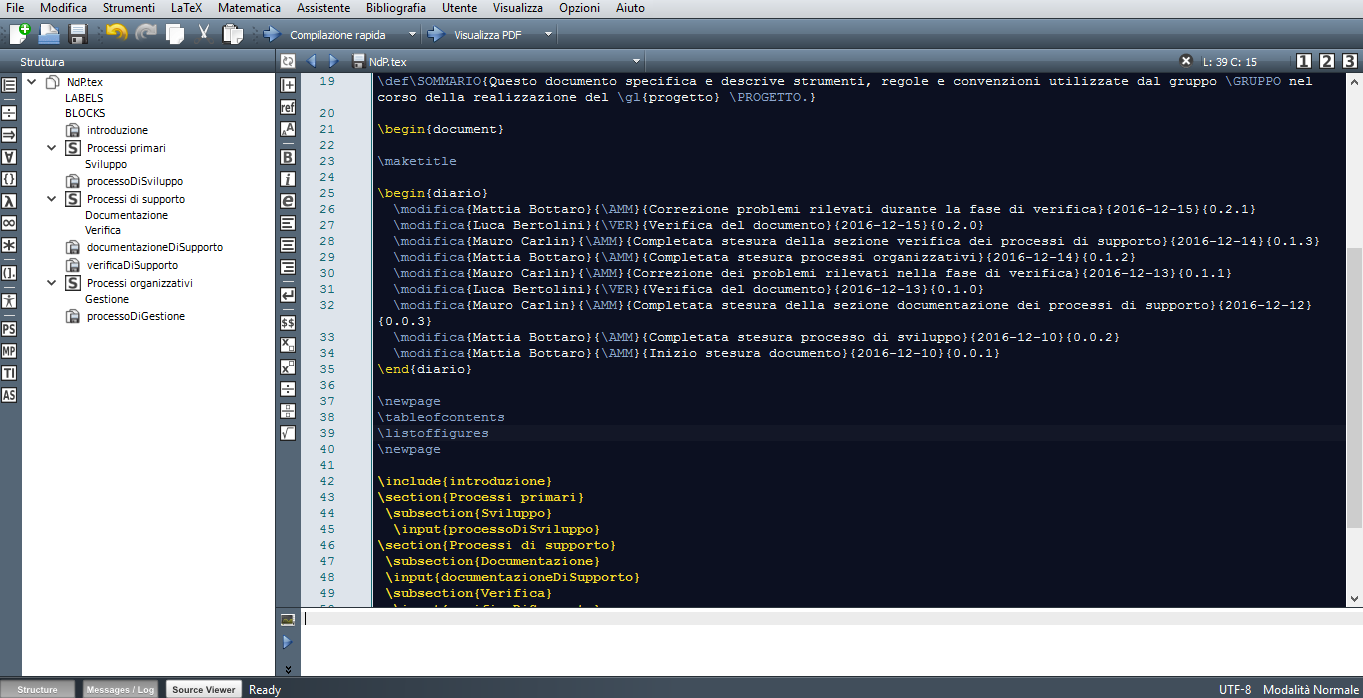
\includegraphics[scale=0.4]{img/texm.png}
\caption{Texmaker}\label{sec:Figura3}
\end{figure}
 \paragraph{Excel}
Per la creazione di grafici (istogrammi, diagrammi a torta, ecc.) viene utilizzato Excel di Microsoft Office, nella versione 2013 o successive.
\paragraph{Script di glossarizzazione}

In \GloScript{} si trova lo script che, per ogni documento, marca come glossarizzate le parole contenute in \file{Docs/template/terminiglossario.txt}, le quali poi saranno presenti nel \Gldoc.
\subsection{Configurazione}
\subsubsection{Versionamento}
\paragraph{Repository}
Per il versionamento e l'archiviazione dei file, l'\AMM{} ha creato un \gl{repository} \gl{GitHub}, il quale è disponibile al seguente indirizzo \url{https://github.com/CoCodeSWE} (visitato in data 2017-02-24). Tutti i membri del gruppo dovranno creare un proprio account GitHub, per poi ricevere i permessi in scrittura sul \gl{repository} da parte dell'\AMM.
La gestione del repository è responsabilità degli \AMMP.
\paragraph{Struttura del repository Docs}
Questo repository è dedicato all'archiviazione dei file per generare tutta la documentazione che il \gl{team} vuole produrre.\\
Al fine di mantenere ordine e coerenza tra i file, il repository è così strutturato:
\begin{itemize}
	\item Docs
	\begin{itemize}
		\item RR
		\begin{itemize}
			\item Esterni: contiene i documenti esterni;
			\item Interni: contiene i documenti interni;
		\end{itemize}
		\item RP
		\begin{itemize}
			\item Esterni: contiene i documenti esterni;
			\item Interni: contiene i documenti interni;
		\end{itemize}
		\item script: contiene gli script utilizzati;
		\item template: contiene i template utilizzati;
	\end{itemize}
\end{itemize}
\paragraph{Struttura del repository \PROGETTO}
Questo repository è dedicato all'archiviazione dei file contenenti il codice sorgente per realizzare il \gl{prodotto}.\\
Al fine di mantenere ordine e coerenza tra i file, il repository è così strutturato:
\begin{itemize}
	\item \PROGETTO
	\begin{itemize}
		\item libs: contiene il codice sorgente di utilizzo comune tra \file{Client} e \file{Back-end};
		\item client: contiene il codice sorgente che realizza la parte \file{Client} del prodotto;
		\item back-end: contiene il codice sorgente che realizza la parte \file{Client} del prodotto;
		\item test: contiene i file che realizzano i test automatici;
	\end{itemize}
\end{itemize}
Questo repository dovrà seguire la gerarchia dei \gl{package} descritta nel documento \DPdoc.
\paragraph{Commit}
Ogni commit effettuata deve essere accompagnata da un messaggio descrittivo delle modifiche effettuate. L'autore della commit dovrà assicurarsi della correttezza dei file. È sconsigliato effettuare il commit di intere cartelle, al fine di evitare inclusioni di file inutili(ad es: file di compilazione).
Dovrà inoltre essere segnalata l'eventuale aggiunta di nuovi file.
\paragraph{Modifiche}
In caso di modifiche importanti da attuare, si dovrà creare un \gl{branch} apposito nel quale lavorare, al fine di proteggere il branch principale di sviluppo. Una volta apportate, le modifiche dovranno essere applicate al branch principale.
\paragraph{Procedure}
\subparagraph{Aggiornamento del repository locale} 
Per aggiornare il repository in oggetto, è necessario seguire la seguente procedura:
\begin{itemize}
	\item aprire il terminale nel repository;
	\item dare il comando \file{git pull}.
\end{itemize}
Se l'operazione non è possibile a causa di conflitti sui file, è necessario risolverli a mano per poi riapplicare la procedura precedente.
\subparagraph{Aggiornamento del repository remoto}
Per aggiornare il repository in oggetto con le proprie modifiche locali, è necessario seguire la seguente procedura:
\begin{itemize}
	\item aprire il terminale nel repository;
	\item dare il comando \file{git add lista\_file} ;
	\item dare il comando \file{git commit -m "messaggio"}, dove il messaggio dovrà essere un breve testo esplicativo delle modifiche che si stanno apportando;
	\item dare il comando \file{git push}.
\end{itemize}
\subparagraph{Utilizzo di un branch}
Per creare un branch è necessario seguire la seguente procedura:
\begin{itemize}
	\item aprire il terminale nel repository;
	\item dare il comando \file{git checkout -b nomeBranch}.
\end{itemize}
Una volta dato \file{git push}, verrà creato il corrispondente branch in GitHub. \\
Una volta terminato il suo utilizzo, il branch dovrà essere eliminato seguendo questa procedura:
\begin{itemize}
	\item aprire il terminale nel repository;
	\item se ci si trova sul branch da eliminare, spostarsi da esso con \file{git checkout master};
	\item dare il comando \file{git checkout -d nomeBranch}.
\end{itemize}
\paragraph{Strumenti}
 \subparagraph{Git}
 Lo strumento usato per il versionamento è Git, in combinazione con il servizio di host GitHub e con GitHub desktop.
 Git è un software open-source di controllo versione distribuito utilizzabile dal terminale. Come versione si utilizza la 2.7.4 o superiori.
 \subparagraph{GitHub}
 GitHub è un servizio di hosting per progetti software, con il quale è possibile interagire tramite Git. GitHub
 offre diversi piani per \gl{repository} privati sia a pagamento, sia gratuiti, molto utilizzati per lo
 sviluppo di progetti open-source. 
 \begin{figure}[h]
 	\centering
 	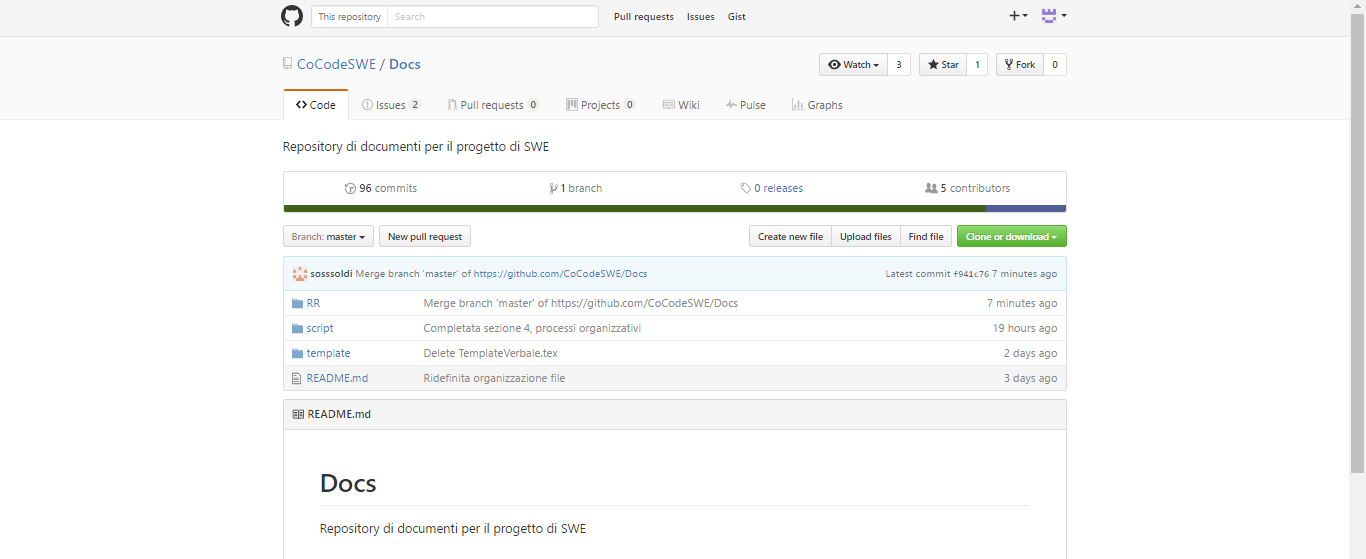
\includegraphics[scale=0.4]{img/github.png}
 	\caption{Github}\label{sec:Figura4}
 \end{figure}
 \subparagraph{GitHub desktop}
 GitHub Desktop è l'applicativo desktop per contribuire e collaborare ai progetti del corrispondente servizio web GitHub. Esso è disponibile per Windows e MacOS. Per Windows si utilizza la versione 3.3.3 o superiori.